\documentclass[a4paper,12pt]{article}
\usepackage{cmap}					% поиск в PDF
% \usepackage{mathtext} 				% русские буквы в формулах
\usepackage[T2A]{fontenc}			% кодировка
\usepackage[utf8]{inputenc}			% кодировка исходного текста
% \usepackage[english,russian]{babel}	% локализация и переносы
% \usepackage[usenames]{color}
% \usepackage{colortbl}
% \usepackage{ifthen}
\usepackage{csquotes} % ещё одна штука для цитат
%%% Дополнительная работа с математикой
\usepackage{amsmath, amsfonts, amssymb, amsthm, mathtools}
% \usepackage{icomma} % "Уная" запятая: $0,2$ --- число, $0, 2$
%% Свои команды
\DeclareMathOperator{\sgn}{\mathop{sgn}}
%% Перенос знаков в формулах (по Львовскому)
\newcommand*{\hm}[1]{#1\nobreak\discretionary{}
{\hbox{$\mathsurround=0pt #1$}}{}}
%%% Работа с картинками
\usepackage{graphicx}  % Для вставки рисунков
% \graphicspath{{images/}{images2/}}  % папки с картинками
% \setlength\fboxsep{3pt} % Отступ рамки \fbox{} от рисунка
% \setlength\fboxrule{1pt} % Толщина линий рамки \fbox{}
\usepackage{wrapfig} % Обтекание рисунков текстом
%%% Работа с таблицами
\usepackage{array,tabularx,tabulary,booktabs} % Дополнительная работа с таблицами
% \usepackage{longtable}  % Длинные таблицы
% \usepackage{multirow} % Слияние строк в таблице
%%% Теоремы
\theoremstyle{plain} % Это стиль по умолчанию, его можно не переопределять.
\numberwithin{equation}{section}
\newtheorem{theorem}{Теорема}[section]
\newtheorem{proposition}[theorem]{Утверждение}
\theoremstyle{definition} % "Определение"
\newtheorem{corollary}{Следствие}[theorem]
\newtheorem{problem}{Задача}[section]
\newtheorem{defn}{Определение}[section]
\theoremstyle{remark} % "Примечание"
\newtheorem*{sol}{\textbf{Решение}}
\newtheorem*{rem}{\textbf{Замечание}}
\usepackage{etoolbox} % логические операторы
%%% Страница
\usepackage{extsizes} % Возможность сделать 14-й шрифт
\usepackage{geometry} % Простой способ задавать поля
	\geometry{top=15mm}
	\geometry{bottom=15mm}
	\geometry{left=15mm}
	\geometry{right=15mm}
 %
%\usepackage{fancyhdr} % Колонтитулы
 %	\pagestyle{empty}
 %	\pagestyle{fancy}
 %	\renewcommand{\headrulewidth}{0mm}  % Толщина линейки, отчеркивающей верхний колонтитул
 %	\lfoot{}
 %	\rfoot{}
 %	\cfoot{}
 %	\rhead{}
 %	\chead{}
 %	\lhead{ }
\renewcommand{\dfrac}[2]{\displaystyle\frac{#1}{#2}}
%\usepackage{setspace} % Интерлиньяж
%\usepackage{lastpage} % Узнать, сколько всего страниц в документе.
%\usepackage{soul} % Модификаторы начертания
\usepackage{hyperref}
\usepackage[usenames,dvipsnames,svgnames,table,rgb]{xcolor}
\hypersetup{				% Гиперссылки
    unicode=true,           % русские буквы в раздела PDF
    pdftitle={Заголовок},   % Заголовок
    pdfauthor={Автор},      % Автор
    pdfsubject={Тема},      % Тема
    pdfcreator={Создатель}, % Создатель
    pdfproducer={Производитель}, % Производитель
    pdfkeywords={keyword1} {key2} {key3}, % Ключевые слова
    colorlinks=true,       	% false: ссылки в рамках; true: цветные ссылки
    linkcolor=red,          % внутренние ссылки
    citecolor=green,        % на библиографию
    filecolor=magenta,      % на файлы
    urlcolor=cyan           % на URL
}
\pagestyle{plain} % нумерация стр вкл.
\usepackage{csquotes} % штука для цитат
\usepackage{multicol} % Несколько колонок
\usepackage{graphicx}
\DeclareGraphicsExtensions{.pdf,.png,.jpg}
\usepackage{cite}
% \usepackage[colorlinks, citecolor=red, urlcolor=blue]{hyperref}
\title{Genetic Algorithm}
\author{Sirazitdinova Zarema}
\date{25 July 2022}
\begin{document}
\large
\maketitle
\tableofcontents
\begin{abstract}
\large
В данном проекте\cite{myers2011art} нами была исследована возможность создания компьютерного приложения, способного самостоятельно находить решение задач на построение с помощью циркуля и линейки в пространстве, на основе на так называемого генетического алгоритма.
\end{abstract}
\section{Введение}
В данном проекте рассматривается возможность создания компьютерного приложения, способного самостоятельно находить решение задач на построение с помощью циркуля и линейки в пространстве.  Разработка данного приложения опирается на так называемый генетический алгоритм, который впервые был применен в 1954 году Нильсом Баричелли на компьютере. Соображения Н. Баричелли были позднее использованы и развиты Алексом Фразером, Давидом Б.Фогелем, Инго Рехенбергем и др. 
В нашем проекте мы создаём виртуальный ГеоМир, обитателями которого являются многогранники, а также виртуальные организмы, названные нами $\gamma$-грызами.$\gamma$-грызы способны строить прямые, а также находить точки пересечения новых прямых с уже построенными (если таковые существуют) с уже построенными. Все построения $\gamma$-грызы выполняют в точном соотвествии с командами, записанными в их генетическом коде.
Изначально создаётся популяция $\gamma$-грызов, генетические коды которых генерируются случайным образом. Затем запускается процесс естественного отбора по следующей схеме.
\begin{itemize}
    \item $\gamma$-грызы пытаются решить задачу, те из них, которые внесли больший вклад в поиск решения задачи получают больше жизненной энергии
    \item  Затем 10\% с наивысшим показателем жизненной энергии дают потомство (часть из них в точности повторяют родителей, а часть – случайным образом мутируют), остальные 90\% вымирают.
    \item появляется новое поколение $\gamma$-грызов
\end{itemize}
 Процесс происходит до тех пор, пока не появится поколение, способное решить задачу. После этого также можно продолжить естественный отбор, для получения оптимального решения.
Для математических расчетов мы выбрали барицентрические координаты в пространстве относительно четырёх заданных точек, намеренно избегая декартовых координат, поскольку мы хотим поставить компьютер в положение ученика, решающего стереометрическую задачу на построения, используя плоский чертёж (проективное изображение стереометрической конструкции на плоскости). Поскольку при проективном преобразовании сохраняется отношение отрезков, лежащих на одной или на параллельных прямых, то барицентрические координаты точек пространства при этом преобразовании относительно четырёх заданных точек сохраняются.
\textbf{Целью проекта} является исследование вопроса возможности применения генетического алгоритма при решении геометрических задач, а также разработка компьютерного приложения, реализующего этот алгоритм.
\textbf{Задачи проекта:}
\begin{enumerate}
    \item изучить литературу и найти информацию в интернете по темам, связанным с проектом;
	\item получить необходимые и достаточные условия в барицентрических координатах, позволяющие	определить	взаимное расположение точек прямых и плоскостей в пространстве;
	\item разработать генетический алгоритм, позволяющий компьютеру самостоятельно решать стереометрические задачи на построение в пространстве;
	\item реализовать разработанный алгоритм в виде компьютерного приложение;
	\item протестировать компьютерное приложение на примере 1-2 конкретных задач.
\end{enumerate}
\textbf{Гипотеза:} Построенный алгоритм может быть использован для решения геометрических задач в разработанном компьютерном приложении.
Данная работа носит теоретико-практический характер. Разработанное нами компьютерное приложение может быть использовано для поиска решения  задач на построение в пространстве, а также в качестве обучающего приложения (например, учитель может использовать данное приложение на уроке, дав ученикам лабораторную работу, на которой ученики,  наблюдая за процессом эволюции $\gamma$-грызов смогут прийти к каким-либо выводам и  тем самым самим обучаться решать предложенные учителем задачи.
\newpage
\section{Необходимые формулы в барицентрических координатах}
\subsection{Понятие центра масс}
В данном разделе рассмотрим понятие центра масс и приведем некоторые его свойства. Пусть точка $A$ -- некоторая точка пространства. Придадим точке $A$ массу $m$, этот факт будем обозначать через $mA$.
Рассмотрим два небольших шарика, имеющих массы $m_1$ и $m_2$, соединенных жестким «невесомым» стержнем. На этом стержне имеется такая замечательная точка $Z$, что если подвесить всю систему в этой точке, то она будет в равновесии -- ни один из шариков не «перетянет». Из физики известно, что эта точка $Z$ и есть центр масс двух рассматриваемых материальных точек с массами $m_1$ и $m_2$ (рис.1). 
\begin{wrapfigure}[16]{r}{0.6\linewidth} 
\vspace{-5ex}
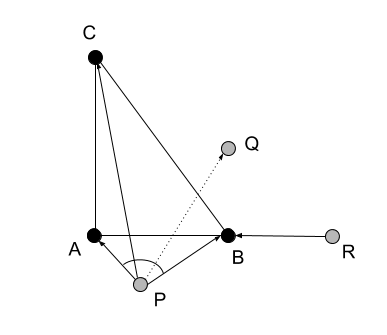
\includegraphics[width=\linewidth]{img/геометрия.png}
\caption{Координаты точек и векторов}
\label{fig:somelabel}
\end{wrapfigure}
Такая же картина наблюдается и для большего числа материальных точек. То есть существует такая $Z$, подвесив за которую всю систему на вертикальной ниточке, а затем как угодно повернув вокруг $Z$, успокоив и отпустив, мы будем наблюдать положение равновесие системы (рис.2).
Но для того, чтобы с помощью понятия центра масс получать математически корректные решения геометрических задач, непригодно определение центра масс с помощью «подвешивания на ниточке». Дадим математическую интерпретацию этого понятия. 
\begin{defn}  Центром масс (или барицентром) системы материальных точек
\begin{equation}\label{syst}
m_1 A_1,m_2 A_2,…,m_n A_n
\end{equation}
называется точка $Z$, для которой имеет место равенство 
\begin{equation}\label{s}
m_1 \overrightarrow{ZA_1}+m_2\overrightarrow{ZA_2}+\ldots+m_n \overrightarrow{ZA_n}=\overrightarrow{0}.
\end{equation}                 
\end{defn}
Центр масс обладает следующим свойством: 
\begin{theorem} Если точка $Z$ служит центром масс системы материальных точек \eqref{syst}, то при любом выборе в пространстве точки $O$ справедливо равенство 
\begin{equation}\label{sy}
    \overrightarrow{OZ}=\dfrac{m_1\overrightarrow{OA_1}+ m_2\overrightarrow{OA_2} +\ldots+m_n\overrightarrow{OA_n}}{m_1+m_2+\ldots+m_n }
\end{equation}
Обратно: 
Если хотя бы при одном выборе в пространстве точки $O$ верно равенство \eqref{sy}, то точка $Z$ -- центр масс системы \eqref{s}.
\end{theorem}
Введем сокращенную запись для \eqref{sy}:  $$Z=\dfrac{m_1A_1+ m_2A_2 +\ldots+ m_nA_n}{m_1+m_2+\ldots+m_n}.$$
Еще одной важной теоремой является правило рычага для двух материальных точек: 
\begin{theorem} Центр масс двух материальных точек (м.т.) расположен на отрезке, соединяющим эти точки; его положение определяется архимедовым правилом рычага: $$m_1\overrightarrow{ZA_1}=m_2\overrightarrow{ZA_2}$$
\end{theorem}
Также запишем теорему о группировке масс: 
\begin{theorem} Пусть в системе(1), состоящей из м.т., отмечены $k$ м.т.$m_1 A_1,m_2 A_2,m_k A_k$ и пусть $C$ – центр масс отмеченных м.т. Если всю массу отмеченных м.т. сосредоточить в их центре масс $C$, то от этого положение центра масс всей системы не изменится. Иначе говоря, система (1)центр, $(m_1+m_2+m_k )C,m_k(+1) A_(k+1) ,m_n A_n. $  [4] 
Массы материальных точек могут быть не только положительными числами (как в физике), но и отрицательными. В этом случае все свойства положительных масс будут сохраняться и для отрицательных [1, гл. I, §2]. 
Рассмотрим систему из трёх м.т.$m_1 A_1,m_2 A_2,m_3 A_3$ и распишем всевозможные вариации расположения центра масс~\cite{Kirsanov20112014Oct} в зависимости от положительных и отрицательных $m_1,m_2 и m_3$ (рис.3).
\end{theorem}
\newpage
\subsection{Барицентрические координаты на плоскости}
Рассмотрим понятие центра масс. Пусть точка $A$ – некоторая точка пространства. Придадим точке $A$ массу $m$, этот факт будем обозначать через $mA$. 
Рассмотрим два небольших шарика, имеющих массы $m_1$ и $m_2$, соединенных жестким «невесомым» стержнем. На этом стержне имеется такая замечательная точка $Z$, что если подвесить всю систему в этой точке, то она будет в равновесии. Из физики известно, что эта точка $Z$ и есть центр масс двух рассматриваемых материальных точек с массами $m_1$ и $m_2$ (рис. 1).
\begin{figure}
\centering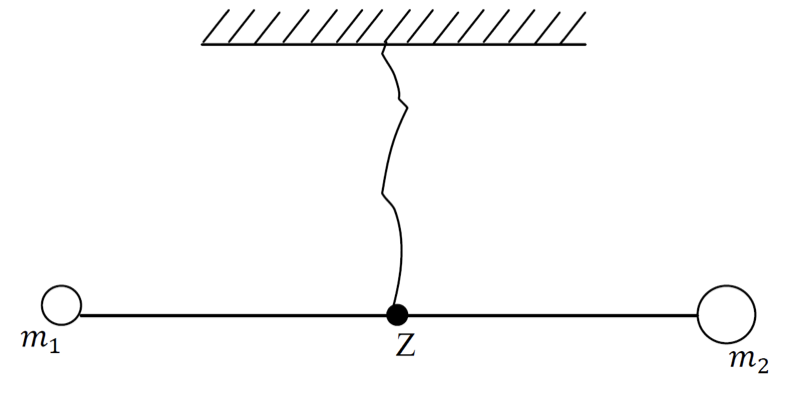
\includegraphics[scale=0.9]{img/центр замечательной точки.png}
\caption{рис.1}
\end{figure}
Такая же картина наблюдается и для большего числа материальных точек. То есть существует такая $Z$, подвесив за которую всю систему на вертикальной ниточке, а затем как угодно повернув вокруг $Z$, успокоив и отпустив, мы будем наблюдать положение равновесие системы (рис. 2).
\begin{figure}[h]
\begin{minipage}[h]{0.49\linewidth}
\center{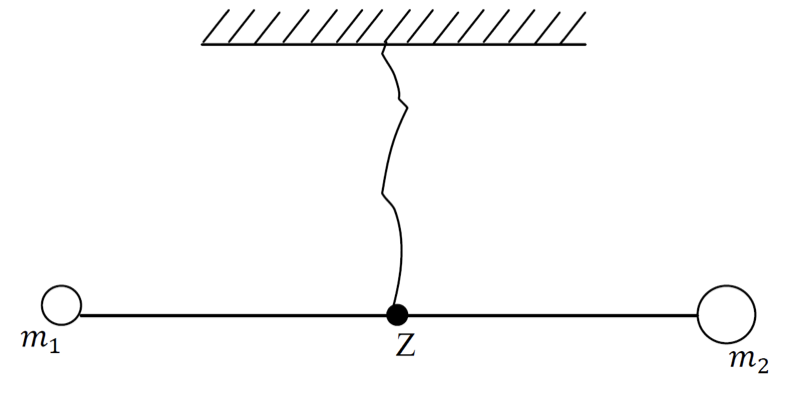
\includegraphics[width=0.7\linewidth]{img/центр замечательной точки.png} \\ а)}
\end{minipage}
\hfill
\begin{minipage}[h]{0.49\linewidth}
\center{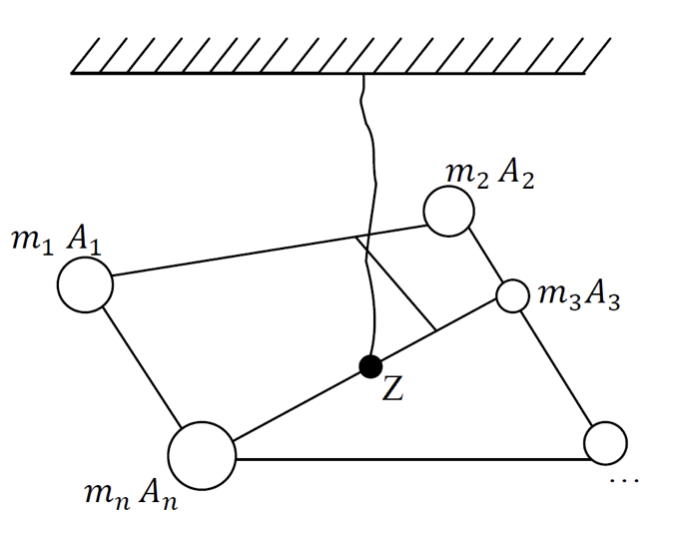
\includegraphics[width=0.7\linewidth]{img/сложная система.png} \\ б)}
\end{minipage}
\caption{рис.2}
\label{ris:image1}
\end{figure}
Но для того, чтобы с помощью понятия центра масс получать математически корректные решения геометрических задач, непригодно определение центра масс с помощью «подвешивания на ниточке». Дадим математическую интерпретацию этого понятия. 
\begin{defn}  Центром масс (или барицентром) системы материальных точек
\begin{equation}\label{syst} m_1 A_1,m_2 A_2,…,m_n A_n
\end{equation}
называется точка $Z$, для которой имеет место равенство 
\begin{equation}\label{s}
m_1 \overrightarrow{ZA_1}+m_2\overrightarrow{ZA_2}+\ldots+m_n \overrightarrow{ZA_n}=\overrightarrow{0}.
\end{equation}                 
\end{defn}
Свойства и выведенные формулы из теорем, которые мы используем в проекте, показаны на доске
\subsection{Барицентрические координаты в пространстве}
\begin{displayquote}
Выберем в пространстве некоторый тетраэдр $A_1A_2A_3A_4$, который в дальнейшем будем называть базисным. 
\end{displayquote}
При любой загрузке четырех вершин тетраэдра действительными массами $m_1, m_2, m_3, m_4$ c ненулевой массой однозначно определена в пространстве точка, являющаяся центром масс этих м.т., и наоборот, для любой точки $P$ возможно подобрать для вершин тетраэдра такие действительные (не обязательно положительные) массы $p_1, p_2, p_3, p_4$ с суммой 1, чтобы центром этих масс оказалась точка $P$. Это доказывается так же, как и на плоскости. Такие числа и будем называть барицентрическими координатами точки $P$.
\begin{enumerate}
    \item (1, 1)
    \begin{enumerate}
        \item (8, 9)
        \item (6, 7) 
        \item (2, 1)
    \end{enumerate}
    \item (5, 9)
    \item (0, 4)
\end{enumerate}
\subsection{ Что такое генетический алгоритм ?}
\begin{displayquote}
\textit{
  Генетический алгоритм – это класс эволюционных алгоритмов поиска.
}
\end{displayquote}
Окружающая среда ГеоМира состоит из точек, прямых, плоскостей и многогранников, а также геометрических задач на построение в пространстве.$\forall x \in X, \quad \exists y \leq \epsilon$
Обитателями ГеоМира являются $\gamma$-грызы, которые «питаются» решением геометрических задач, получая от их решения жизненную энергию по законам, изложенным далее. Мы будем использовать генетический алгоритм для решения стереометрических задач на построения с помощью циркуля и линейки~\cite{Anna2019Jun}. Например, для заданного тетраэдра и заданных точек на ребрах или гранях тетраэдра построить пересечения заданной прямой с заданной плоскостью, пересечение двух заданных плоскостей, построение сечение тетраэдра и т.д. 
Для этого создадим «существ», которых мы назвали $\gamma$-грызами (от греческого "геометрия" и от выражения «грызть гранит науки»). 
$\gamma$-грыз – виртуальный «организм» генетический код которого, состоит из массива (последовательности) генов. Каждый ген представляет из себя неупорядоченную пару различных неотрицательных целых чисел. К примеру, генетический код $\gamma$-грыза Жорика выглядит так:
\begin{center}
\begin{tabular}{ccc}
Первая координата: & \textbf{(0, 5)} \\
Вторая координата: & \textbf{(0, 4)} \\
Третья координата: & \textbf{(4, 5)} \\
\end{tabular}
\end{center}
Каждый ген отвечает за построение какой-либо прямой в пространстве. Если $\gamma$-грыз встречает геометрическую задачу на построение, то он начинает «грызть» по следующей схеме:
\begin{enumerate}
    \item $\gamma$-грыз определяет список точек, прямых и базовых плоскостей. Каждой точке присваивается номер, начиная с нуля;
	\item Сначала срабатывает первый ген. Потом последовательно срабатывают все последующие гены;
	\item Каждый ген строит прямую, проходящую через точки с номерами, записанными в этих генах. А затем находят точки пересечения этой прямой с уже имеющимися прямыми (если таковые существуют). После этого добавляет новые прямую и точки в список, также новым точкам присваивают следующие номера.
\end{enumerate}
В самом начале у $\gamma$-грыза жизненная энергия равна 100 условным единицам. За каждый шаг построения его жизненная энергия уменьшается на 2 условных единицы.  За каждую новую точку $\gamma$-грыз получает 3 условных единицы энергии, если эта точка лежит на ребре, 2 условных единицы, если точка лежит на базовой плоскости, 1 условная единица во всех остальных случаях. Если задача решена, то $\gamma$-грыз получает 1000 условных единиц энергии плюс максимальное значение энергии всех $\gamma$-грызов, не решивших эту задачу. За свою жизнь один $\gamma$-грыз может сгрызть только одну геометрическую задачу. После чего он умирает либо оставляя потомство, либо исчезает без следа.Потомство могут оставить только $\gamma$-грызов с наивысшим показателем жизненной энергии. Остальные  умирают, не оставляя потомство.Каждый $\gamma$-грыз из первой десятки порождает порождаю ровно  копий самого себя, то есть  новых $\gamma$-грызов генетический код которых в точности совпадает с генетическим кодом родителя. Правда у трёх из них может произойти от 1 до 3 случайных мутаций генов. То есть  потомков данного $\gamma$-грыза генетический код будет идентичен коду родителя, а у трёх потомков генетический код будет случайным образом слегка изменён, почти совпадая с кодом родителя. Каждый потомок в момент рождения получит жизненную энергию, равную  условным единицам.Случайная мутация очень важна, так как позволяет создавать $\gamma$-грызов с новым генетическим кодом. Если в результате мутации мы получим более худший экземпляр, то он вымрет в результате естественного отбора, если же появится лучший экземпляр, то он станет доминировать в популяции, только улучшая показатели.
\newpage
\begin{tabular}{c r @{.} l}
Мутация $\pi$       &
\multicolumn{2}{c}{$\gamma$-грыза} \\
\hline
$\pi$               & 9&17  \\
$\pi^{\pi}$         & 8&457   \\
$(\pi^{\pi})^{\pi}$ & 6042&1 \\
\end{tabular}
В данном проекте нами была рассмотрена возможность создания компьютерного приложения\cite{BibEntry2022Jul}, способного самостоятельно находить решение задач на построение с помощью циркуля и линейки в пространстве\footnote{Данная работа носит теоретико-практический характер. Разработанное нами компьютерное приложение, может быть использовано для поиска решения  задач на построение в пространстве, а также в качестве обучающего приложения}, на основе на так называемого генетического алгоритма.
\bibliographystyle{plain}
\bibliography{references.bib}

\begin{wrapfigure}[14]{l}{0.6\linewidth} 
\vspace{-0.5ex}
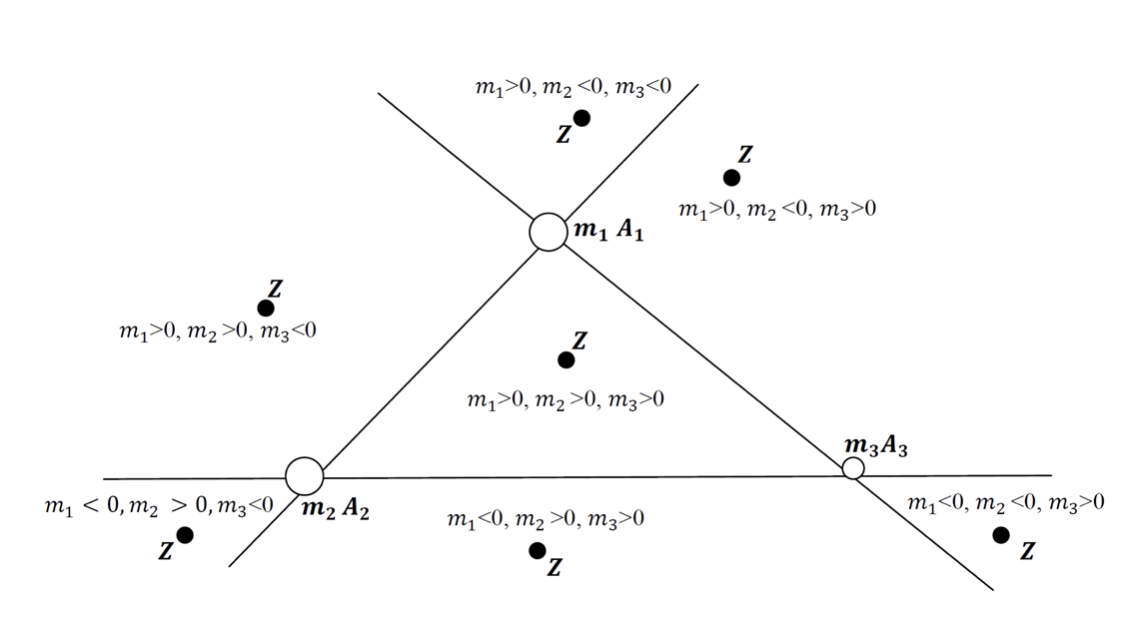
\includegraphics[width=\linewidth]{img/координаты.png}
\label{fig:somelabel}
\end{wrapfigure}

\end{document} % конец документа
